% Packages
\documentclass[11pt,a4paper]{article}
\usepackage[utf8]{inputenc}
\usepackage[T1]{fontenc}
\usepackage{hyperref}
\usepackage{lmodern}
\usepackage[english]{babel}
\usepackage{appendix}
\usepackage{enumitem}

%Fusionneer des pages
\usepackage{pgfpages}
%\pgfpagesuselayout{4 on 1}[a4paper,border shrink=5mm]

% Taille marges
\usepackage[left=2cm,right=2cm,top=2cm,bottom=2cm]{geometry}
% Titles size
\usepackage[small]{titlesec}

% math
\usepackage{amsfonts}
\usepackage{amsmath}
\usepackage{amssymb}
\usepackage{mathabx}
\usepackage{stmaryrd}

\usepackage[most]{tcolorbox}
\newtcolorbox[auto counter]{definition}[1]{colframe=red!75!black, coltitle=white, enhanced, frame empty, colback=white,fonttitle=\bfseries , title=Def \thetcbcounter$\;$: #1, borderline west={2pt}{0pt}{red!85!black},
attach boxed title to top left={xshift=-5mm}, boxed title style={colback=red!75!black}}

\newtcolorbox[auto counter]{prop}{colframe=black!80!white, coltitle=black, enhanced, frame empty, colback=white,fonttitle=\bfseries , title=\underline{Property \thetcbcounter$\;$:}, borderline west={2pt}{0pt}{black},
attach boxed title to top left={xshift=-4mm}, boxed title style={frame empty,colback=white}}

\newtcolorbox[auto counter]{thm}[1]{colframe=blue!70!black,colback=white,fonttitle=\bfseries , title=Theorem \thetcbcounter$\;$: #1}

\newtcolorbox[auto counter]{exercice}{colframe=white,colback=white,fonttitle=\bfseries , title=Exercice \thetcbcounter$\;$:}

\newtcolorbox{preuve}{boxrule=0pt, enhanced, colback=white, colframe=white, coltitle=black, fonttitle=\bfseries , title=\underline{Proof $\;$:},
top=0mm, frame empty, borderline west={1pt}{0pt}{black}, sharp corners,
after upper={\par\hfill\textit{$\blacksquare $}}}

\newtcolorbox{mybox}{colframe=white!75!black,colback=white!95!black,fonttitle=\bfseries}

% pseudo code
\usepackage[ruled,lined,noend]{algorithm2e}
\usepackage{babel}

% insertion image
\usepackage{graphicx}
\graphicspath{ {./images/} }

% derivation tree
\usepackage{ebproof}

% automate
\usepackage{caption}
\usepackage{tikz}
\usetikzlibrary{automata, positioning, arrows, decorations.pathreplacing, decorations.markings, positioning, shapes, quotes}


\newcounter{fig}
\newcommand{\fig}[3]{
	\begin{center}
	\begin{figure}[ht]
		\refstepcounter{fig}
		\centering
		\begin{tikzpicture}[scale=#3]
		#1
		\end{tikzpicture}
		\caption{\underline{#2}}
	\end{figure}
	\end{center}
}

\newcommand{\tab}{\phantom{xxx}}

\newcommand{\ignore}[1]{}

\newcommand{\uao}[3]{\underset{#1}{\overset{#2}{#3}}}

\renewcommand{\lim}[2]{\underset{#1 \rightarrow #2}{lim}}

\newcommand{\mlist}[1]{\begin{itemize}[noitemsep,topsep=0pt]#1\end{itemize}}



\title{\vspace{-1.0cm}Performance Evaluation project:\\\underline{Optimizing cars' trajectory with AI}}
\date{}
\author{\vspace{-1cm}Ottavy Macéo, Longatte Mathieu, Louison Mocq}

\begin{document}
\maketitle
%\tableofcontents

	\part{Introduction}
The goal of this project is split into five parts:
\mlist{
\item Creating racing car environment to simulate simple 2D racing car model.
\item Implementing Deep Q-learning and Genetic algorithms to optmize the behaviour of a car on trakcs so that the car can have the best trajectories possible.
\item Evalute the performances of Deep Q-learning and Genetic algorithms and compare them.
\item Evalute the performances of Deep Q-learning depending of the hyperparameters.
\item As a bonus: evaluate the performance of our best car's behaviour.
}
All the code have been made with python.

	\part{Deep Q-learning}
		\section{Markovian decision porcess}
		
		\section{What is Q value?}
		
		\section{What is Q learning}

	
	\part{Genetic algorithms}
		\section{What are genetic algorithms}
		
		\section{Markov Chain modelisation}
		
		\section{NEAT}
	
	
	\part{Car Racing environment}
		\section{Tracks}
A track is originally a .png file wich look like the left image of figure \ref{figure:track}. Then, the image is converted to a matrix $T$ such that $T[0][0]$ is the bottom left corner. After that, we crop the image, compute the starting point and the lines of track (that will be explained in the reward part) to have a final result which look the right image of figure \ref{figure:track}.
\begin{center}
\label{figure:track}
	\begin{figure}[ht]
		\refstepcounter{fig}
		\centering
		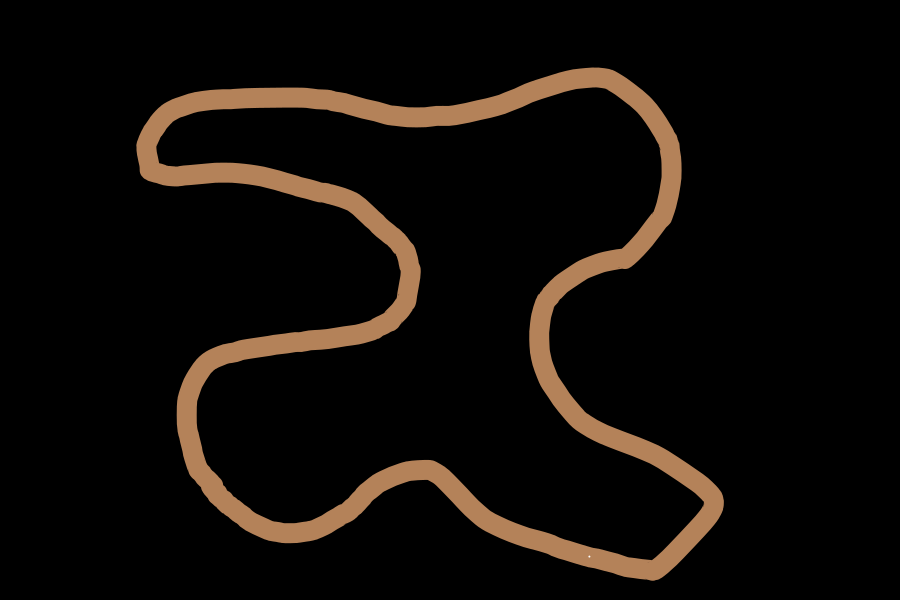
\includegraphics[width=5cm, height=4cm]{track_06.png}
		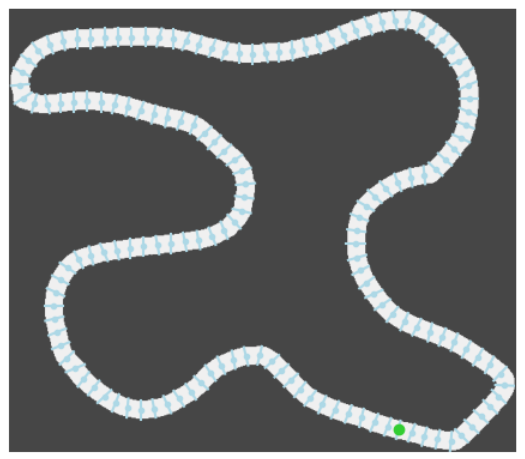
\includegraphics[width=5cm, height=4cm]{track_06_computed.png}
		\caption{\underline{.png and computed track}}
	\end{figure}
\end{center}

	
		\section{Cars' physics}
The Car physic is really simple. It is a 2D cartoon-like physics that act as follow:\\
The car has to main informations: its speed $\in [0,$ MaxSpeed$]$ and its rotation $\in [0,360]$. The physics is simple, at each times step, the car move to next coordinates on direction of the car's rotation and of a lenght equal to the car's speed.\\
If the coordinates of the car is $(x,y)$, its speed is $s$ and its rotation is $\alpha$, then, after a time step, the coordinate of the car will be:
\[(s.cos(\frac{\pi}{180}\alpha) + x,\; s.sin(\frac{\pi}{180}\alpha) + x)\]
\\
Moreover, at each time step, the car can make some actions:
\mlist{
\item it can accelerate, this will increase the car's speed by a constant
\item it can brake, this will decrease the car's speed by reduce the car speed by a constant. The car cannot have a negative speed.
\item it can turn, i.e. add a constant $\in \llbracket-K,K\rrbracket$ to its rotation. $K$ is a constant that is the maximum angle the car can turn per each time step.
}
		
		\section{Technical aspects of the environment}
To manipulate our environment, we use the python packages \texttt{gymnasium} which provide code convention for those type or environment, i.e. environment where at each time step, you have one action to do. The environment has to have
		
		\section{Rewards}
	
	
	\part{Performance Evaluation}
		\section{Algorithms}
		
		\section{Best car}



\end{document}